\documentclass[a4paper]{article}
% \documentclass[a4paper]{book}

% Imports
\usepackage[utf8]{inputenc}
\usepackage[ngerman]{babel}
\usepackage{fancyhdr}
\usepackage{caption}
\usepackage{float}
\usepackage{subcaption}
\usepackage{epigraph}
\usepackage[acronym]{glossaries}
\usepackage{graphicx}
%\usepackage{pdfpages}
%\usepackage{attachfile2}
\usepackage{tabularx}
\usepackage{cite}
\usepackage{hyperref}

% Generate the glossary
\makeglossaries

% Title page
\title{Open Source Software \\
    \noindent\rule[0.25ex]{\linewidth}{0.5pt}
    \large Wie nehmen Endanwender Open Source Software wahr?
}

\author{
  Blechschmidt, Til\\
  \texttt{til@blechschmidt.de}\\
  Nordakademie, Elmshorn
  \and
  Peeters, Noah\\
  \texttt{noah.peeters@icloud.com}\\
  Nordakademie, Elmshorn
}

% Numbering
\setcounter{secnumdepth}{3}
\setcounter{tocdepth}{2}

% Quote styling
\setlength\epigraphwidth{.8\textwidth}
\setlength\epigraphrule{0pt}

% Glossary
% \newglossaryentry{oss}{name=OSS, description={Open Source Software}}
\newacronym{oss}{OSS}{Open Source Software}


\begin{document}
    % Title page
    \thispagestyle{fancy}
    \maketitle

    % Abstract
    \clearpage
    \begin{abstract}
         \gls{oss} wird in vielen Bereichen eingesetzt. In dieser Arbeit wird analysiert, wie Endanwender \gls{oss} wahrnehmen.
    \end{abstract}
    \newpage

    % TOC
    \tableofcontents
    \listoffigures
    \listoftables
    \clearpage

    % --- Content ---
    
                    
    \section{Fragestellung}
        In der Arbeit soll die Frage, inwiefern Endanwender Open Source Software wahrnehmen, untersucht werden. Dabei soll nicht nur die \emph{direkte} Verwendung von Open Source Software, wie es zum Beispiel bei LibreOffice der Fall ist, eine Rolle spielen, sondern auch die \emph{indirekte} Nutzung als Komponente kommerzieller Lösungen wie Chromium als Basis von Google Chrome\footnote{Genaue Definitionen sind in \ref{section:indirekte_nutzung} zu finden.}
		
		Es wird erwartet, dass viele Nutzer unbewusst und indirekt mit Open Source Software in Kontakt stehen, sie diese also als Teil größerer, kommerzieller Closed Source Software nutzen, sich dessen aber nicht bewusst sind. Außerdem ist zu erwarten, dass nur ein kleiner Teil der Anwender direkt mit Open Source Software interagiert\cite{oss:lotus-to-linux}.
		
		Um zuverlässige Daten zu erhalten, die die aktuelle Wahrnehmung der Endanwender widerspiegeln, wurde eine Umfrage durchgeführt. Für die Sicherstellung der Repräsentativität der Umfrage wurden mindestens 80 Antworten erwartet.
		Die Umfrage wurde quantitativ mit geschlossenen Fragen gestaltet, um den Aufwand für die Befragten zu minimieren und damit die Teilnehmerrate und Datenmenge zu maximieren. % TODO: Cite
		
		\subsection{Definitionen} % TODO: Achtung Reihenfolge Definitionen/Fragestellung
            \subsubsection{Open Source Software}
                \begin{quote} 
                    \centering 
                    Software wird als Open Source bezeichnet, wenn ihr Quelltext frei zugänglich ist. Sie kann in kommerzieller Software eingesetzt werden, ihre Nutzung muss allerdings nicht kostenfrei sein. 
                \end{quote}
                
            \subsubsection{Nutzung von Open Source Software}\label{section:indirekte_nutzung}
                Die Nutzung von Open Source Software durch Endanwender kann in zwei Arten unterschieden werden.
                
                \paragraph{Direkte Nutzung}
                    Zum einen gibt es die direkte Nutzung, bei der der Nutzer eine Software verwendet, die Open Source ist, also dessen Source Code frei zugänglich ist.
                    
                    Beispiele für Direkte Nutzung:
                    \begin{itemize}
                        \item Wikipedia\footnote{Wikipedia ist eine Konfiguration von Wikimedia, dessen Source Code frei zugänglich ist.}                        \item Thunderbird % TODO add reference to table
                        \item ... % TODO: mehr Beispiele
                    \end{itemize}
                    
                \paragraph{Indirekte Nutzung}
                    Zum anderen gibt es die indirekte Nutzung. Hier verwendet der Nutzer Software, dessen Source Code nicht frei zugänglich ist, deren Funktionalität aber entscheidend von \gls{oss} Komponenten abhängt. Ohne diese Komponenten wäre die Funktionalität stark eingeschränkt. Hierbei werden folgende Komponenten \textbf{nicht} berücksichtigt:
                    
                    \begin{itemize}
                        \item Entwicklerwerkzeuge wie Compiler
                        \item Datenbanken wie MySQL
                        \item Betriebssysteme wie Linux 
                        \item ... 
                    \end{itemize} % TODO: gibt es mehr? Apache Web server?
                    Der Grund dafür liegt in der Verbreitung dieser Komponenten. % TODO: bessere Erklärung
                    
                    Beispiele für Indirekte Nutzung:
                    \begin{itemize}
                        \item Google Chrome % TODO add reference to table
                        \item macOS % TODO add reference to table
                        \item ... % TODO: mehr Beispiele
                    \end{itemize}

            
        
    \section{Design und Durchführung}
		Zweck der Befragung ist es, einen repräsentativen Überblick über die Wahrnehmung von Open Source Software des Endanwenders zu erhalten. Dabei soll Aufschluss über die Verteilung von indirekter sowie direkter Nutzung gegeben werden und in dem Zusammenhang analysiert werden, warum sich Anwender für Open Source Software entscheiden. Außerdem soll evaluiert werden, welche Gründe die Nutzer für und gegen die Nutzung von Open Source Software sehen.
	
		\subsection{Design}
		  \subsubsection{Aufbau}
    			Die Erhebung ist in vier Teile gegliedert, die im Folgenden näher erläutert sind: 
    		   
    			\paragraph{Bewusste Nutzung}
    				Um die, dem Anwender bewusste, Nutzung von Open Source Software zu erheben, beginnt die Umfrage mit diesem Abschnitt.\\
    				Zunächst wird ermittelt, ob die Nutzer wissen, was Open Source Software ist. Um im weiteren Verlauf der Umfrage sinnvolle Antworten zu erhalten, wird anschließend die Definition von Software sowie quelloffener Software erklärt.\\
    				Nun werden Fragen zum Nutzungsverhalten von solcher Software gestellt ohne dabei Beispiele zu nennen, um Beeinflussung zu vermeiden.
    			
    			\paragraph{Unbewusste Nutzung}
    				Im zweiten Abschnitt werden konkrete Beispiele für Open Source Software genannt, um die Nutzer darauf aufmerksam zu machen, wo Open Source Komponenten und Softwares überall eingesetzt werden, ohne dass es ihnen klar ist.\\
    				Außerdem soll geklärt werden, warum es Differenzen, wenn vorhanden, zwischen bewusster und unbewusster Nutzung gibt.
    			
    			\paragraph{Gründe für und gegen Open Source Software}
    				Im dritten Abschnitt werden Fragen bezüglich der Nutzungs- und Hinderungsgründe von Open Source Software gestellt. Dazu wird gefragt, warum oder warum nicht Endnutzer oder Unternehmen Open Source Software einsetzten. Die möglichen Antworten werden aus der Schweizer Studie zum Thema Open Source\cite{oss:studie} genommen, um die Wahrnehmung mit der realen Nutzung vergleichbar zu machen.
    			
    			\paragraph{Demographische Differenzen}
    				Zur Analyse von Differenzen innerhalb der Bevölkerungen enthält die Umfrage Fragen zur aktuellen Tätigkeit\footnote{Schüler, Student, Arbeitnehmer, etc.} sowie zur Selbsteinschätzung der Computerkenntnisse.
				
			\subsubsection{Designentscheidungen}
			 \begin{itemize}
			     \item Es wurde überwiegend auf Freifelder verzichtet, um die Auswertung zu vereinfachen. Deshalb wurde bei dem eingesetzten Freifeld ein einheitliches Format gefordert.
				\item Bei Skalen wurde darauf geachtet eine gerade Anzahl an Optionen anzubieten, um den Nutzer nicht die Möglichkeit zu bieten neutral zu antworten.
				\item Die Texte sollen möglichst allgemeinverständlich geschrieben sein, um auch Nutzern ohne technischen Hintergrund die Teilnahme an der Umfrage zu ermöglichen.
			 \end{itemize}
			     
		\subsection{Durchführung}
            \subsubsection{Verbreitung}
                Um die Reichweite der Umfrage zu maximieren und die Kosten zu minimieren wurde diese in Form einer Onlinebefragung umgesetzt. Dabei wurden Kanäle wie Social Media, E-Mail, Messenger genutzt, um auf die Umfrage aufmerksam zu machen. Zudem wurde der Link zu der Umfrage über private Kontakte und an der Nordakademie verbreitet.
                
    \section{Auswertung}
        \subsection{Vorgehen}
            \paragraph{Auswertung des Freifeldes}
                Um mit den Daten des Freifeldes zu arbeiten, wurden zunächst alle Begriffe, die die Nutzer eingegeben haben, einer Kategorie zugeordnet. Alle Begriffe, denen kein sinnvoller Inhalt zugeordnet werden konnte, wurden in der Kategorie '-' zusammengefasst. Diese Zuordnung ist in der Tabelle \ref{table:categories} auf Seite \pageref{table:categories} dargestellt.\\
            
            \begin{table}[h]
                \begin{tabularx}{\textwidth}{rX}
                    Kategorie & Begriffe \\
                    \hline
                    - & \tiny geht, ?, hilfee, komische, privat, , !, nutze, wissentlich, nix, ibt, immer noch nicht verstanden was es ist, weil, keine ahnung, .., ich, blub, frage, tue, meist ohne opensource, benutze, modell, ..., warum ist das hier pflichtfeld?, bla, es sie g, nicht, ohne, und, ich nicht\\
                    Alternativlos & \tiny alternativlos, keine alternative\\
                    Anpassbarkeit & \tiny vielfältigkeit, man kann selber eingreifen, teilweise anbassbar, zeitvertreib, benutzerindividuell, vielseitig, offen für eigene entwicklungen, anpassbarkeit, erweiterbar, kontrolle, flexible, individuell, kompatibler, erweiterungen, anpassbar, variantenreich\\
                    Auswahl & \tiny auswahl\\
                    Benutzerfreundlichkeit & \tiny sympathisch, verwaltung, schön, einfach, moderrn, freundlich zu bedienen, handhabbar, anwendungsnutzen, verständlich\\
                    Code Veränderbarkeit & \tiny änderbar, veränderbar, offener quelltext\\
                    Community & \tiny jeder kann mitmachen, community, große community, wurde empfohlen, demokratisch, communitysupport, guter support/foren, verbreitet, communitydriven, großer nutzenkreis, anleitungen, community"", sozial, viel hilfestellung im internet, oft verbreitet\\
                    Datenschutz & \tiny vertrauenswürdigkeit, datenschutz, privatsphäre, datensicherheitt\\
                    Entwickler Community & \tiny mit pacman installierbar, updatefrequenz, schnellere sofwareentwicklung, große entwickler gemeinschaft\\
                    Erfahrung & \tiny erprobt, erfahrung, gewohnheit\\
                    Frei & \tiny offene standards, freiheit, verifizierbar, keine geheimnisse, quellcode, open standard, frei, openess, freiheit (fsf)\\
                    Funktionalität & \tiny teilweise mehr funktionen als normale programme, weils funktioniert, funktionalität, funktionsbereitstellung\\
                    Grundeinstellung & \tiny gutes gefühl, prinzip, open source unterstützen, moralischer, überzeugung, weltanschauung, moral, philosophie\\
                    Hilfreich & \tiny hilfreich\\
                    Indirekte Nutzung & \tiny fast überall ist oss enthalten\\
                    Innovation & \tiny innovativ, kreativ, gutes konzept, innovation\\
                    Kompatibilität & \tiny kompatibel, kompatibilität\\
                    Kosten & \tiny free, teilweisekostenfrei, kostenvorteil, kostenlos, gratis, billig, kostengünstig, günstig, kostenersparnis, kosten, umsonst, preis, preiswert, oft kostenlos, for free, kostenfrei, häufig kostenlos, meistens kostenlos, meist kostenlos\\
                    Notwendig & \tiny arbeit, notwendigkeit, abeit\\
                    Nützlich & \tiny praktisch, nützlich\\
                    Qualität & \tiny teilw. besser, oft gute alternative, besser als kommerzielle sw, besser, gute alternative, gut, stabilität, plattformunabhängig, ""schlechter"" als nicht open source, meistens aktuell, funktioniert, aktuell, zuverlässig, zielorientierung, qualität, schnell, stable, fast genauso wie vergleichbare programme, oft besser, manchmal besser, toll, fehlerfreiheit\\
                    Sicherheit & \tiny ""sicher, sicher, sicherheit, sicherer\\
                    Testversion & \tiny testversion\\
                    Transparenz & \tiny transparent, transparant, transparenz, offen\\
                    Unabhängigkeit & \tiny unabhängigkeit, keine großen konzerne unterstützen, against microsoft, unabhängig von herstellern, anti-kommerz, unabhängig\\
                    Unbewusste Nutzung & \tiny unbewusst\\
                    Verfügbarkeit & \tiny schneller zugriff, einfach zu bekommen, verfügbarkeit, freizugänglich, leicht zugänglich, schnell verfügbar als download, gut zugänglich, verfügbar\\
                    Vertrauen & \tiny vertrauen\\
                    Weiterentwicklung & \tiny weiterentwicklung\\
                    Zufall & \tiny keine gründe, hat keinen speziellen grund, zufall, weil software die ich brauche zufällig open-source ist\\
                \end{tabularx}
                \caption{Zuordnung der Begriffe des Freifeldes zu Kategorien}
            \label{table:categories}
            \end{table}
            
            Im späteren Verlauf der Arbeit werden die Werte des Freifelds mit den Ergebnissen einer Schweizer Studie verglichen. Dazu bedarf es einer Zuordnung zu den vorliegenden Kategorien aus der Studie, welche in Tabelle \ref{table:privateToCommercialCategories} dargelegt ist.\\
            
            \begin{table}
                \centering
                \bgroup
                \def\arraystretch{1.5}
                \begin{tabular}{ r | l }
                    Freifeld Kategorie & Schweizer Studie\\ \hline
                    Kosten & Kosteneinsparungen\\
                    Anpassbarkeit & Anpassbarkeit\\
                    Unabhängigkeit & Unabhängigkeit\\
                    Grundeinstellung & Offene Standards\\
                    Transparenz & Transparenz\\
                    Community & Community\\
                    Innovation & Innovation\\
                    Sicherheit & Sicherheit\\
                    Weiterentwicklung & Mitarbeitende\\
                    Qualität & Stabilität
                \end{tabular}
                \egroup
                \caption{Zuordnung | Freifeld $\leftrightarrow$ Schweizer Studie}
                \label{table:privateToCommercialCategories}
            \end{table}
            
        \subsection{Validität der Ergebnisse}
            - Ausreichender Stichprobenumfang
            - Stichprobe fokussiert auf Studenten und Arbeitstätige mit guten Computerkenntnissen. Renter und Schüler sowie Leute mit wenigen Computerkenntnissen sind wenig vertreten

    \section{Ergebnisse}
        \subsection{Wissen über OSS}
            \begin{figure}
                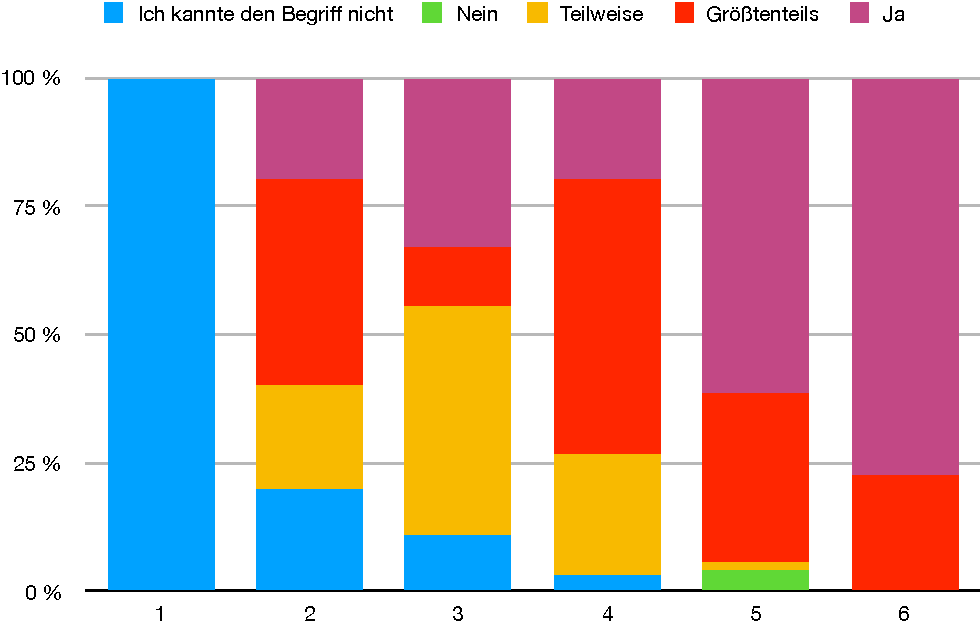
\includegraphics[width=\textwidth]{assets/results/definition/definition.pdf}
                \caption{Korrektheit der eigenen Definition nach Selbsteinschätzung geordnet.}
            \end{figure}
        
            \begin{figure}
                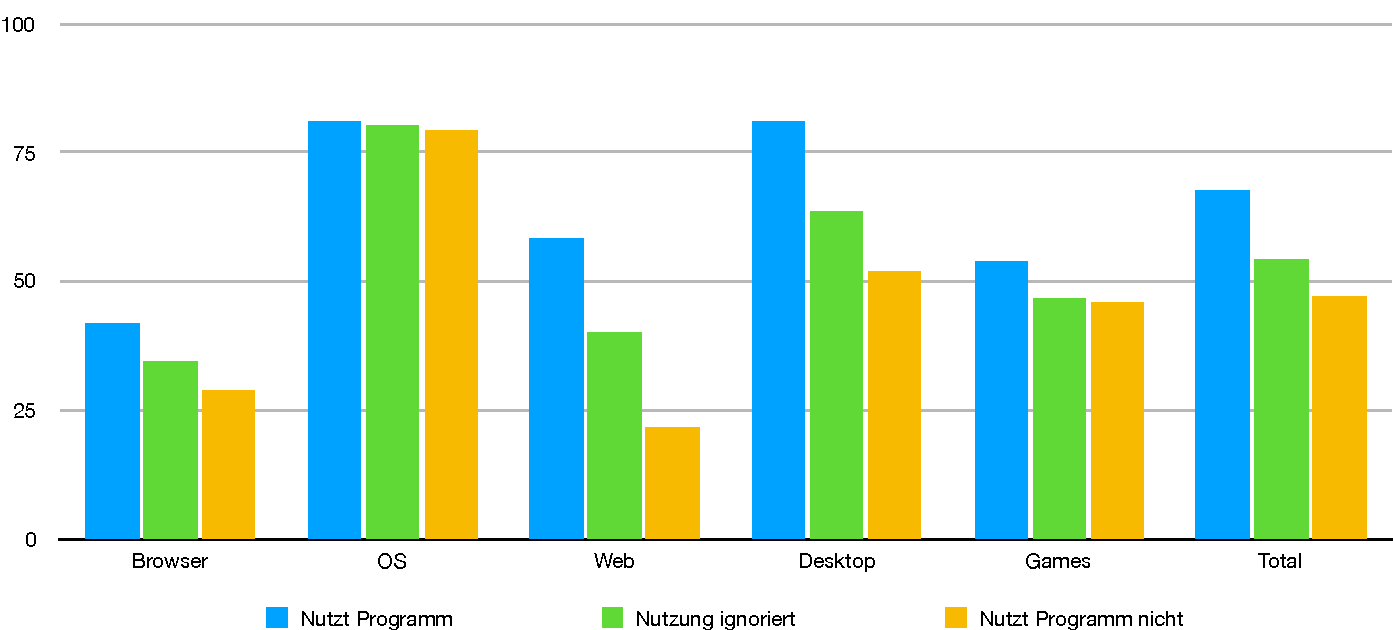
\includegraphics[width=\textwidth]{assets/results/openSourceJudging/openSourceJudging}
                \caption{Attribut Open Source  |  unbeeinflusste Nutzereinschätzung}
            \end{figure}
            Das Wissen über Open Source Software bei Endanwendern ...
            
        \clearpage
        \newpage
        \subsection{Nutzungsgründe für Open Source Software}
            Im Jahr 2015 führte die Forschungsstelle Digitale Nachhaltigkeit des Instituts für Wirtschaftsinformatik an der Universität Bern eine Befragung von 200 Schweizer Unternehmen durch\cite{oss:studie}. Eins der Ziele der Umfrage war es, ein Ranking der Nutzungsgründe von \gls{oss} für Unternehmen aufzustellen.

            \paragraph{Sicht der Nutzer auf Unternehmen}
                Um einen Einblick in die Sicht der Nutzer auf Unternehmen zu bekommen wurden die Endanwender befragt, welches die drei signifikantesten Gründe für den Einsatz von \gls{oss} in Unternehmen sind. Dabei wurden die gleichen Kategorien wie in der Eingangs erwähnten Studie in einer Multiple-Choice Frage abgefragt.

            \paragraph{Privat}
                Zusätzlich ist von Interesse, was die privaten Gründe für die Nutzung von Open Source Anwendungen sind. Dazu gab es in der Umfrage ein Freifeld, wo nach den drei wichtigsten Gründen für den privaten Einsatz von \gls{oss} gefragt wurde. Diese wurden anschließend grob kategorisiert\footnote{Siehe Tabelle \ref{table:categories} auf Seite \pageref{table:categories}.} und anschließend den Kategorien der Schweizer Studie zugeordnet.
                
            \begin{figure}
                % TODO Trendline in graph is broken
                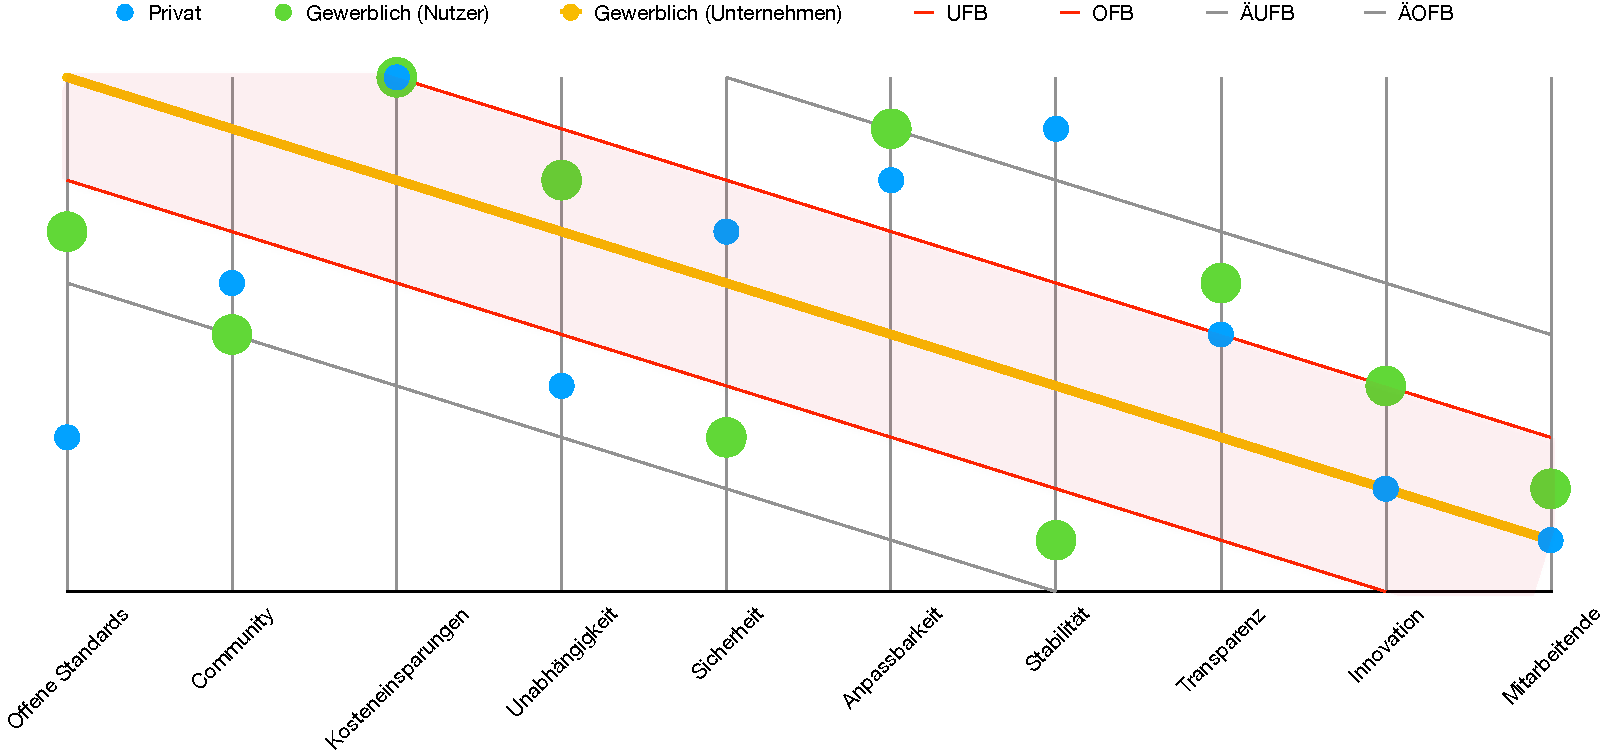
\includegraphics[width=\textwidth]{assets/results/commercialReasoning/usageReasonRanking}
                \caption{Ranking der Nutzungsgründe}
                \label{table:usageRanking}
            \end{figure}
                
            \subsubsection{Aufbau des Diagramms}
                \paragraph{Kategorien}
                    Auf der x-Achse des Diagramms sind die Kategorien, welche der Schweizer Studie entnommen wurden, nach ihrer Wichtigkeit für Unternehmen von links nach rechts in absteigender Reihenfolge angeordnet.
                    
                \paragraph{Rankings}
                    Die y-Achse des Diagramms stellt die Wichtigkeit eines Aspekts für die Nutzung von \gls{oss} dar. Ein höherer Wert korrespondiert hierbei zu einer größeren Wichtigkeit.
                    
                \paragraph{innerer Fehlerbereich}
                    Der rot markierte Bereich stellt den inneren Toleranz- bzw. Fehlerbereich dar, welcher alle Werte mit einer Abweichung von dem Ranking der Unternehmen von maximal zwei einschließt. Sämtliche Datenpunkte, die sich in diesem Bereich befinden werden im folgenden als \"richtig\" angesehen, da ihre Abweichung von dem Zielwert nur gering ist.
                    
                \paragraph{äußerer Fehlerbereich}
                    Der Bereich zwischen den roten und grauen Linien wird im folgenden als äußerer Toleranz- bzw. Fehlerbereich genannt. Er beinhaltet alle Werte, dessen absolute Abweichung von dem Ranking der Unternehmen mehr als zwei und maximal vier entspricht.
                    
                \paragraph{Datenpunkte}
                    Das Diagramm beinhaltet drei verschiedene Werte für jede der Kategorien, wobei die Größe der Punkte keinerlei Bedeutung hat und lediglich dazu dient überlappende Punkte sichtbar zu machen. Im folgenden bezeichnen Datenpunkte ausschließlich die Werte, welche im Graphen grün eingezeichnet sind. Die Farben sind wie folgt zugeordnet:\\
                    \begin{table}[H]
                        \centering
                        \bgroup
                        \def\arraystretch{1.5}
                        \begin{tabular}{ r | l }
                            \emph{Blau} & private Nutzung aus Sicht der Endanwender\\
                            \emph{Grün} & gewerbliche Nutzung aus Sicht der Endanwender\\
                            \emph{Gelb} & tatsächliche gewerbliche Nutzungsgründe
                        \end{tabular}
                        \egroup
                    \end{table}
                    
                    Die Quellen der einzelnen Datensätze sind im Folgenden erläutert:
                    \subparagraph{private Nutzung} Wie Eingangs erwähnt wurde das Freifeld in der Umfrage nach Tabelle \ref{table:categories} gegliedert und diese anschließend den Kategorien der Studie zugeordnet. Diese Zuordnung ist in Tabelle \ref{table:privateToCommercialCategories} einzusehen.
                    
                    \subparagraph{Sicht der Nutzer auf Unternehmen} Die Antworten der Multiple-Choice Frage bezüglich des Rankings wurden kumuliert und darauf basierend ein Ranking erstellt.
                    
                    \subparagraph{gewerbliche Nutzung} Das Ranking für die gewerbliche Nutzung wurden Figur 8 auf Seite 16 der Schweizer Studie\cite{oss:studie} direkt entnommen.
            
            \subsubsection{Auswertung des Diagramms}
                \paragraph{Sicht der Nutzer auf Unternehmen}
                    Abbildung \ref{table:usageRanking} kann man entnehmen, dass sich $40\%$ der Datenpunkte im inneren Fehlerbereich befinden ({\scriptsize Kosteneinsparungen, Unabhängigkeit, Innovation, Mitarbeitende}) und somit als richtig anzusehen sind. Komplementär dazu befinden sich $60\%$ der Datenpunkte im äußeren Fehlerbereich und \emph{keine} Datenpunkte außerhalb der Fehlerbereiche.\\
                    Dabei ist zu beachten, dass $20\%$ der Kategorien oberhalb ({\scriptsize Anpassbarkeit, Transparenz}) und $40\%$ unterhalb ({\scriptsize Offene Standards, Community, Sicherheit, Stabilität}) des inneren Toleranzbereichs liegen.
                    
                \paragraph{Abweichung von privaten Gründen}
                    Des weiteren ist auffällig, dass $60\%$ der Werte innerhalb des Toleranzbereichs\footnote{Der Toleranzbereich um die privaten Gründe ist im Diagramm nicht verzeichnet, hat aber die gleiche Toleranz wie der der gewerblichen Gründe und lässt sich daher nachmessen.} von den privaten Gründen liegen, wovon sich die Hälfte der Datenpunkte in dem inneren Fehlerbereich befindet.
                               
            \subsubsection{Interpretation der Daten}
                \paragraph{Abweichung von der Realität}
                    Betrachtet man den äußeren Toleranzbereich, so liegen die Nutzer mit ihrer Einschätzung grob richtig. Schaut man nun allerdings auf den inneren Fehlerbereich, so liegen nur noch $40\%$ der Kategorien mit ihrem Ranking in der unmittelbaren Nähe der Schweizer Unternehmen. Dies lässt darauf schließen, dass die allgemeine Ansicht welche Aspekte für Unternehmen von Bedeutung sind vorhanden, jedoch nicht stark ausgeprägt sind.\\
                    Des Weiteren ist auffällig, dass die Aspekte \emph{Offene Standards} und \emph{Stablität} welche sich in Relation zu den privaten Gründen in die richtige Richtung orientieren beide zu schwach eingeschätzt wurden.
                    
                \paragraph{Projektion privater Gründe}
                    Schaut man sich die Werte ausserhalb des inneren Fehlerbereichs an, so fällt auf, dass $50\%$ der Punkte ({\scriptsize Community, Anpassbarkeit, Transparenz}) eine sehr geringe Distanz zu den privaten Gründen haben. Daraus lässt sich ableiten, dass die Nutzer möglicherweise ihre privaten Gründe auf Unternehmen projizieren.\\
                    Betrachtet man ebenfalls die Werte innerhalb des Toleranzbereichs, so findet man weitere Beispiele, welche diese These ({\scriptsize Kosteneinsparungen, Innovation, Mitarbeitende}) unterstreichen. Es lässt sich anhand der vorliegenden Daten allerdings nicht zweifelsfrei beweisen, dass die Punkte lediglich aufgrund der Projektion und nicht aufgrund des Wissens der Nutzer in dem inneren Fehlerbereich liegen.\\
                    Nimmt man alle Datenpunkte die eine maximale Abweichung von zwei zu den privaten Nutzungsgründen haben und geht davon aus, dass diese ihre aktuelle Position aufgrund der Projektion haben, so bleibt lediglich ein Punkt in dem inneren Toleranzbereich übrig. Dies ist der Aspekt der \emph{Unabhängigkeit}, welcher eindeutig von den Nutzern richtig in den inneren Toleranzbereich eingeordnet wurde.
                    
                    \clearpage
    
    \section{Zusammenfassung}
        \subsection{Verbesserungen am Fragebogen}
            % TODO
            \begin{itemize}
                \item In Umfrage sollte man nicht "Ja/Nein" sondern "Ja/Nein/Keine Ahnung" machen. Evtl. auch die maximal mögliche Signifikanz dessen erörtern.
            \end{itemize}
            
        \subsection{Fazit}
            % TODO
        
    
    \clearpage
    \section{Eidesstaatliche Erklärung}
        Hiermit erklären wir, dass wir die vorliegende Hausarbeit selbstständig verfasst und keine anderen als die angegebenen Hilfsmittel benutzt haben.\\
        Die Stellen der Hausarbeit, die andere Quellen im Wortlaut oder dem Sinn nach entnommen wurden, sind durch Angabe der Herkunft kenntlich gemacht. Dies gilt auch für Zeichnungen, Skizzen, bildliche Darstellungen sowie für Quellen aus dem Internet.
        
        
        \begin{figure}[H]
            \centering
            \begin{minipage}{.5\textwidth}
                \centering
                
\includegraphics[width=\textwidth]{assets/signature_tilb.png}
                Til Blechschmidt
                \label{fig:test1}
            \end{minipage}%
            \begin{minipage}{.5\textwidth}
                \centering
                
\includegraphics[width=\textwidth]{assets/signature_noahp.png}
                Noah Peeters
                \label{fig:test2}
            \end{minipage}
        \end{figure}
        \clearpage
    
    \clearpage
    \section{Appendix}
        \printglossary[type=\acronymtype]
        \printglossary
        
        \clearpage
        \nocite{*}
        \bibliographystyle{unsrt}
        \bibliography{Bibliography}
        
        \clearpage
        
        \subsection{Abschnitte}
            \begin{tabular}{rl}
              Abschnitt & Autor \\
              \hline
              Bla & N. Peeters\\
              Bla & T. Blechschmidt
            \end{tabular}
        
%        \subsection{Umfrage}
%            \paragraph{Ergebnisse}
%                Die Ergebnisse der Umfrage liegen als CSV-Datei bei und sind auch in dieses PDF eingebunden: \attachfile{assets/Open Source.csv}
%            \paragraph{Fragebogen}
%                Auf den nächsten vier Seiten befindet sich eine PDF-Version des Fragebogens, wie er Online verbreitet wurde.
%                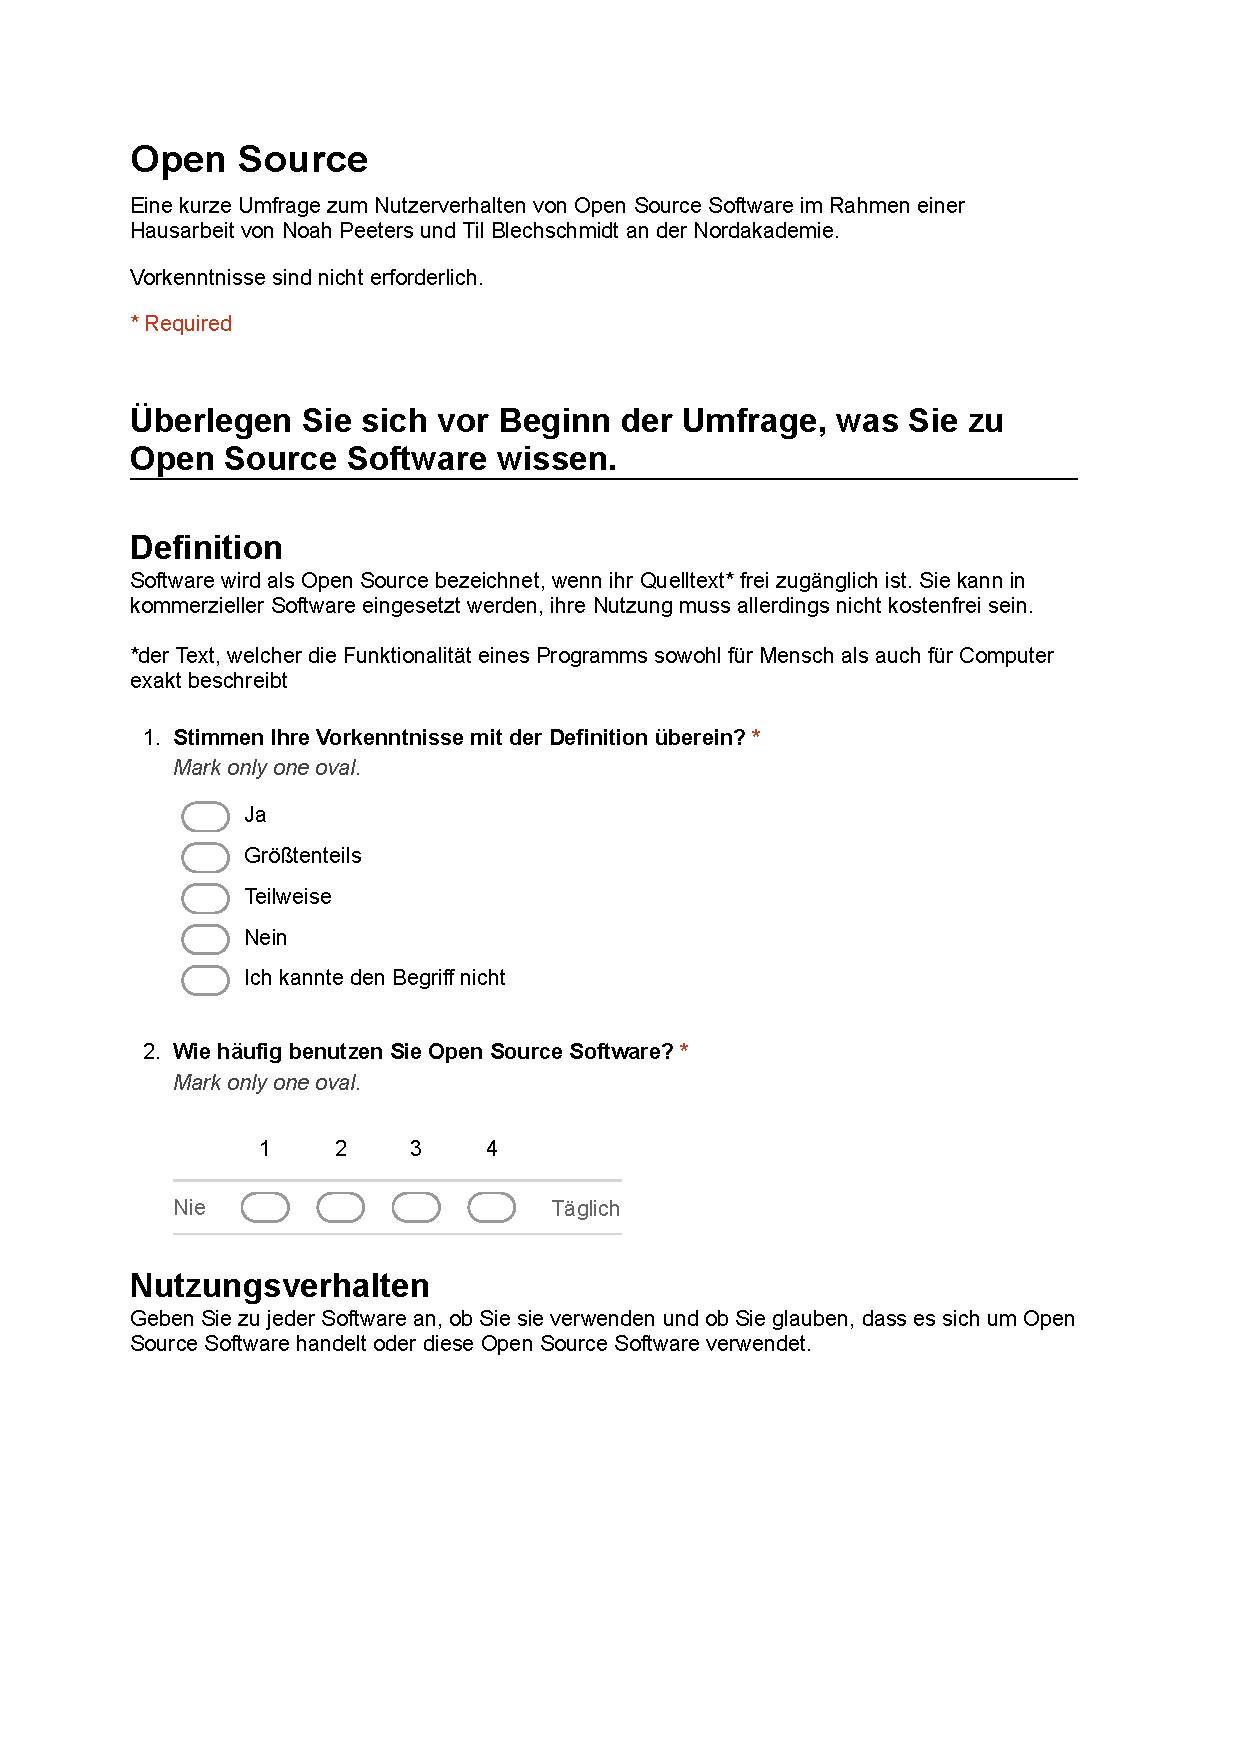
\includepdf[pages={-}]{assets/Umfrage.pdf}

\end{document}
